\documentclass[a4paper,fleqn]{cas-sc}
\usepackage[authoryear]{natbib}
\usepackage{lineno}
\usepackage{booktabs}
\usepackage{url}
\linenumbers

\begin{document}
\let\WriteBookmarks\relax
\def\floatpagepagefraction{1}
\def\textpagefraction{.001}

\shorttitle{MODIS net photosynthesis across a tropical hydroclimatic gradient}
\shortauthors{Y.A.S. Oliveira et al.}

\title[mode = title]{Regularized polynomial regression of MODIS net photosynthesis across a tropical hydroclimatic gradient: Atlantic Forest, Cerrado and Caatinga in northeastern Brazil (2001--2025)}

\author[1]{Ygor Augusto dos Santos Oliveira}[orcid=0000-0000-0000-0000]
\cormark[1]
\ead{ygornayty2@gmail.com}
\credit{Conceptualization, Methodology, Software, Formal analysis, Data curation, Writing -- original draft}

\author[1]{Nayanne Silva Benfica}
\credit{Conceptualization, Methodology, Data curation, Writing -- review \& editing, Supervision}

\author[1]{Fabr\'icio Berton Zanchi}
\credit{Conceptualization, Methodology, Writing -- review \& editing, Supervision}

\affiliation[1]{organization={Graduate Program in Environmental Sciences and Technologies, Federal University of Southern Bahia / Federal Institute of Education, Science and Technology of Bahia},
  city={Porto Seguro},
  postcode={45810-000},
  state={Bahia},
  country={Brazil}}

\cortext[1]{Corresponding author}

\begin{abstract}
The Atlantic Forest, Cerrado and Caatinga biomes of Bahia State respond differently to climate, and these responses are rarely linear. This study developed and validated a multiple polynomial regression model, estimated by Ridge regression, for monthly net photosynthesis (PSN) of the three biomes between 2001 and 2025, using MODIS products and GPM IMERG precipitation. Candidate predictors were evapotranspiration, precipitation, land surface temperature, a water availability index and burned area, together with two harmonic components of the annual cycle. Polynomial degree and predictor set were selected by repeated cross-validation, and both the selection and the performance were verified by year-grouped validation, chronological blocks and null models that preserve the temporal structure of the series. The degree-2 model explained 96.7\% of PSN variance in the Cerrado, 94.2\% in the Caatinga and 73.7\% in the Atlantic Forest, with a maximum drop of 6.7 points under chronological validation. In the Cerrado, the water availability index was selected in place of temperature in the best-performing combination, with a small but consistent difference across partitions; in the Atlantic Forest, it contributed only through interactions with evapotranspiration and temperature. Removing the harmonic components lowered performance by 21.8 points in the Atlantic Forest and by less than 3 points in the seasonal biomes, and showed that the apparent contribution of precipitation largely reflects the annual cycle. The results characterize three distinct patterns of association between climate and productivity and indicate that regularized polynomial regression is a reproducible and interpretable alternative for vegetation monitoring with remote sensing data.
\end{abstract}

\begin{highlights}
\item Degree-2 Ridge polynomial explained 97\%, 94\% and 74\% of monthly PSN in three biomes
\item Degree, predictor set and performance held under year-grouped and chronological validation
\item In the Cerrado, the water availability index was selected in place of temperature
\item With explicit seasonality, predictor contribution reflects anomalies, not the calendar
\item Three association patterns: water limitation, pulsed response and multifactorial response
\end{highlights}

\begin{keywords}
MODIS \sep Net photosynthesis \sep Ridge regression \sep Seasonality \sep Brazilian biomes \sep Temporal validation
\end{keywords}

\maketitle

\section{Introduction}\label{sec:intro}

Net photosynthesis (PSN) is the carbon assimilated by vegetation after subtracting the maintenance respiration of leaves and fine roots and therefore responds almost immediately to environmental conditions \citep{running2004,running2021gpp}. At the monthly scale, PSN is a more direct indicator of photosynthetic activity than annually integrated net primary production and has been used to track vegetation responses to climatic and anthropogenic factors \citep{nemani2003,benfica2023}. The Atlantic Forest, Cerrado and Caatinga biomes of Bahia State are conservation priorities subjected to distinct pressures: forest fragmentation and silviculture along the coast, expansion of the agricultural frontier in the western Cerrado, and degradation and desertification in the semi-arid interior \citep{ribeiro2009,lima2020,marengo2018,mapbiomas2025}. For these biomes, \citet{benfica2022,benfica2023} showed that PSN correlates positively with evapotranspiration and with a water availability index and negatively with land surface temperature, with greater climatic sensitivity in the Cerrado and Caatinga.

These relationships, however, are rarely linear. Productivity increases with water availability only up to a point, beyond which it saturates or declines, and empirical studies document precipitation thresholds below which productivity responds more strongly \citep{jin2018,linger2020,mwangi2025}. More broadly, theoretical ecology describes ecosystems as complex systems with critical transitions and context dependence \citep{levin1998,flores2024}, and IPCC assessments stress that responses to combined pressures involve thresholds and interactions \citep{ipcc2022}. Among non-linear alternatives, machine learning methods have dominated remote-sensing estimates of productivity, with good predictive performance but little transparency about the shape of the fitted relationships. Multiple regression with polynomial and interaction terms occupies an intermediate position: it accommodates curvature and combined effects among predictors while keeping interpretable coefficients. Its classical limitation, the multicollinearity generated by the polynomial expansion itself, is handled by Ridge regression, which penalizes coefficient magnitude and stabilizes estimation \citep{hoerl1970}. Polynomial regression protocols with combinatorial term selection and Y-randomization testing are established in quantitative structure--activity modelling in medicinal chemistry \citep{guimaraes2024}, but their application to monthly vegetation productivity series, with the temporal validation such series require, has not yet been explored.

This study aims (1) to develop and validate a Multiple Polynomial Regression Model of order N (MPRM-N), estimated by Ridge regression, for monthly PSN of the Atlantic Forest, Cerrado and Caatinga biomes of Bahia between 2001 and 2025; (2) to determine empirically the polynomial degree and the set of environmental variables with the best generalization in each biome, under validation schemes that respect the chronological order of the data; and (3) to compare the climatic associations of PSN among the biomes, assessing how the explicit representation of the annual cycle changes the interpretation of predictor contribution.

\section{Materials and methods}\label{sec:methods}

\subsection{Study area}

The Atlantic Forest, Cerrado and Caatinga biomes are located in Bahia State, northeastern Brazil, and occupy about 19\%, 27\% and 54\%, respectively, of the 564,764~km$^2$ of the state \citep{ibge2004,ibge2025} (Fig.~\ref{fig:map}). According to the K\"oppen classification for Brazil \citep{alvares2013}, the coast and the east of the state, under the Atlantic Forest, have a humid tropical climate; the interior and the north, under the Caatinga, have a semi-arid climate with annual precipitation between about 240 and 1,500~mm; and the west and the south, under the Cerrado, have a tropical climate with a well-defined dry season. The Atlantic Forest is dominated by mosaics of forest remnants interspersed with pasture, cocoa agroforestry, eucalyptus plantations and urban areas; in the west of the state, the MATOPIBA agricultural frontier has converted large areas of Cerrado into cropland and pasture; and in the Caatinga, extensive cattle ranching, rainfed agriculture and firewood extraction account for most of the conversion of native vegetation \citep{mapbiomas2025}.

\begin{figure}
  \centering
  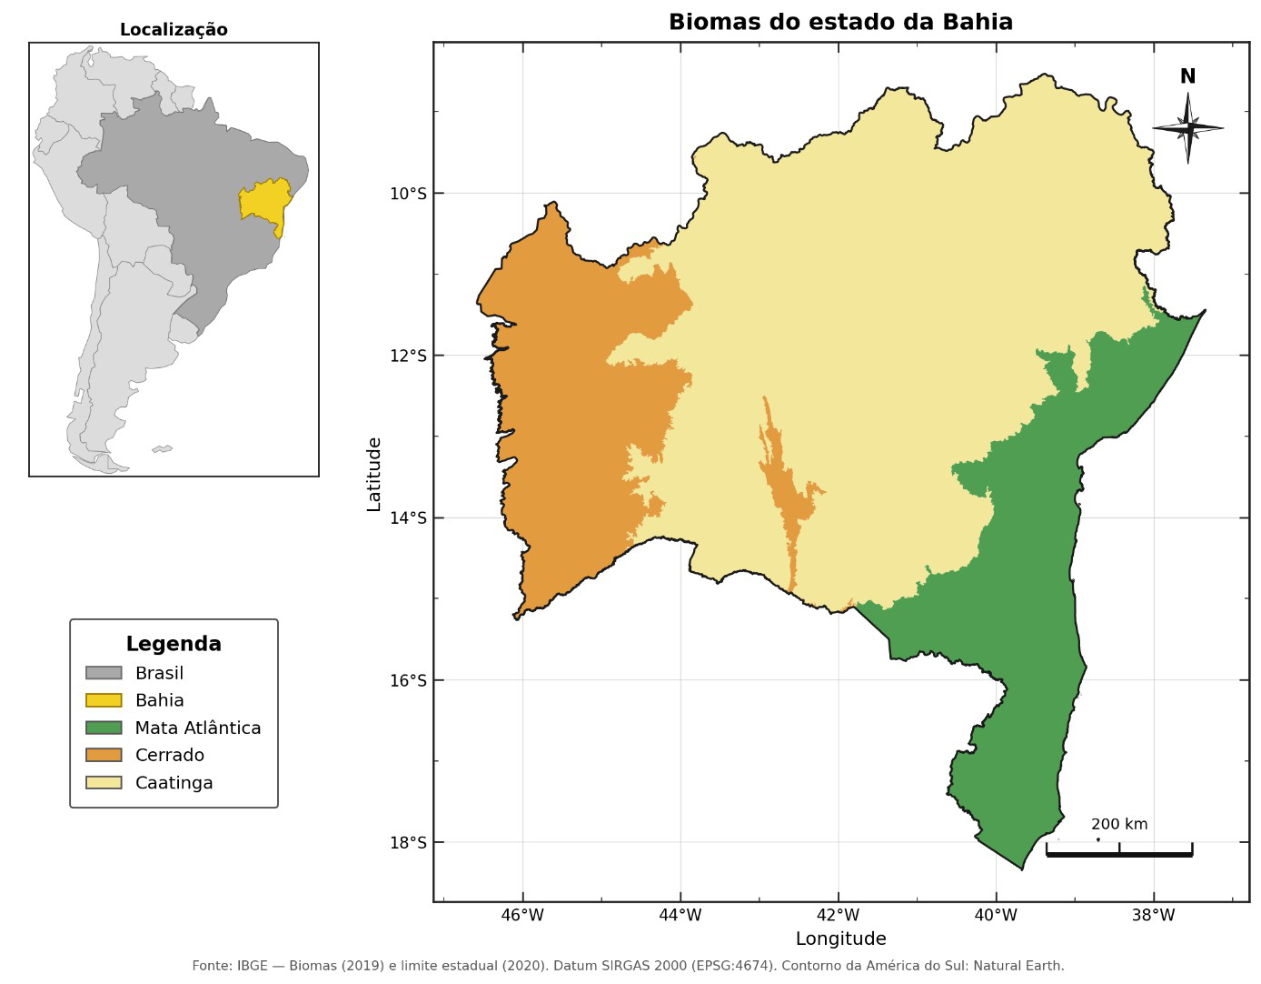
\includegraphics[width=0.8\textwidth]{figs/fig1_map.png}
  \caption{Location and distribution of the Atlantic Forest, Cerrado and Caatinga biomes in Bahia State, Brazil \citep[boundaries from][]{ibge2019}.}\label{fig:map}
\end{figure}

\subsection{Net photosynthesis, climatic variables and burned area}

PSN was obtained from the MOD17A2HGF product and actual (EV) and potential (PET) evapotranspiration from MOD16A2GF, both from Collection 6.1 of the MODIS/Terra sensor, in eight-day composites at 500~m spatial resolution and in their gap-filled versions \citep{running2021gpp,running2021et}. Land surface temperature (LST) was obtained from the daytime band of MOD11A2 at 1~km \citep{wan2021} and burned area (BURN) from the monthly MCD64A1 product \citep{giglio2018}. Precipitation (PRE) was obtained from the monthly GPM IMERG Final Run product, version 07, at 0.1$^\circ$ \citep{huffman2023}, which replaced version 06 used by \citet{benfica2023}. All products were retrieved and processed in Google Earth Engine \citep{gorelick2017}.

For each composite, the spatial mean of valid pixels was computed within each biome, delimited by the IBGE biome map at 1:250,000 scale \citep{ibge2019} clipped to the state boundary, using the official scale factors of each product. Pixels within the valid range of each product were retained. For the gap-filled products (MOD17A2HGF and MOD16A2GF) no additional quality-flag filter was applied, because these versions already replace low-quality observations with interpolated values \citep{running2021gpp}, which does not remove the uncertainty inherent to these products. MOD11A2 has no gap-filled version: pixels without a clear-sky observation receive no LST value and are excluded from the composite mean, but the QC\_Day quality band, which classifies the uncertainty of the retained pixels, was not used as a filter, and the sensitivity of the LST series to this filter was not evaluated (see limitations in the Discussion). Composites were aggregated into fixed windows of four consecutive composites, about 32 days, reproducing the aggregation of \citet{benfica2022,benfica2023}: PSN, EV and PET were summed and LST was averaged in each window. Each window was assigned to the calendar month containing most of its days (January, for example, comprises the composites starting on 27 December and on 1, 9 and 17 January), and the seasonal components are associated with that reference month; the periods referred to here as monthly are therefore fixed 32-day windows rather than strict calendar months, which keeps comparability with the original series. The water availability index (WAI) was computed as the EV/PET ratio and burned area as the number of burned pixels in the month multiplied by pixel area. The series spans January 2001 to September 2025 ($n = 297$ months per biome); the last three months of 2025 were excluded because NASA discontinued IMERG version 07 in September 2025 \citep{nasa2026}. Reproduction of the \citet{benfica2023} database by this procedure yielded correlations above 0.97 with the original series for all variables, and the annual sum of PSN correlated at 0.99--1.00 with annual NPP from the independent MOD17A3HGF product. Variables are described in Table~\ref{tbl:vars}.

\begin{table}[htbp]
\caption{Response variable and candidate predictors of the MPRM-N.}\label{tbl:vars}
\begin{tabular*}{\tblwidth}{@{}LLLL@{}}
\toprule
Variable & Description & Unit & Source \\
\midrule
PSN & Net photosynthesis (response) & gC\,m$^{-2}$\,month$^{-1}$ & MOD17A2HGF \\
EV & Actual evapotranspiration & mm\,month$^{-1}$ & MOD16A2GF \\
PRE & Accumulated precipitation & mm\,month$^{-1}$ & GPM IMERG V07 \\
LST & Daytime land surface temperature & $^\circ$C & MOD11A2 \\
WAI & Water availability index (EV/PET) & dimensionless & MOD16A2GF \\
BURN & Burned area, transformed as $\log(1+x)$ & ha & MCD64A1 \\
SAZsin, SAZcos & Harmonic components of the annual cycle & dimensionless & Derived from month \\
\bottomrule
\end{tabular*}
\end{table}

\subsection{Multiple polynomial regression model}

The MPRM-N follows the polynomial regression architecture of \citet{guimaraes2024}, adapted to the environmental context by three decisions: estimation by Ridge regression with L2 regularization instead of ordinary least squares; empirical determination of the polynomial degree between 1 and 5; and extension of the validation protocol with temporal schemes. The general form of the model is given by Eq.~(\ref{eq:model}), where $\hat{Y}$ is the estimated PSN, $X_i$ are the standardized predictors, $\beta_i$ are the linear coefficients and $\beta_{ij}$ and $\beta_{ijk}$ the coefficients of quadratic and interaction terms. Coefficients are estimated by minimizing the penalized loss function of Eq.~(\ref{eq:loss}), where $\alpha$ controls the L2 penalty.
\noindent\begin{minipage}{\columnwidth}
\begin{align}
\hat{Y} &= \beta_0 + \sum_i \beta_i X_i + \sum_{i \le j} \beta_{ij} X_i X_j \nonumber\\
        &\quad + \sum_{i \le j \le k} \beta_{ijk} X_i X_j X_k + \dots \label{eq:model}\\
L(\beta) &= \sum_{n=1}^{N} \left(Y_n - \hat{Y}_n\right)^2 + \alpha \sum_{p=1}^{P} \beta_p^2 \label{eq:loss}
\end{align}
\end{minipage}
\vspace{0.5\baselineskip}

Predictors comprise three environmental variables, selected among EV, PRE, LST, WAI and BURN, and two harmonic components of the annual cycle, $\mathrm{SAZsin} = \sin(2\pi\,\mathrm{month}/12)$ and $\mathrm{SAZcos} = \cos(2\pi\,\mathrm{month}/12)$, kept fixed in all models. Since $\beta_1\,\mathrm{SAZsin} + \beta_2\,\mathrm{SAZcos}$ equals $A\sin(2\pi\,\mathrm{month}/12 + \varphi)$, the model freely fits the amplitude and phase of the annual cycle without imposing artificial relations between months. For five predictors and degree 2, the expansion yields 20 terms (5 linear, 5 quadratic and 10 pairwise interactions); for a generic degree N, the number of terms is $\binom{5+N}{N} - 1$, i.e. 55, 125 and 251 terms for degrees 3 to 5. Before modelling, burned area was transformed as $\log(1+x)$, PET was excluded as a predictor because of its 0.73--0.80 correlation with LST, and the PSN of the training set was winsorized at the 3rd percentile to reduce the influence of months with abnormally low productivity, while test values were kept on their original scale; sensitivity to this choice was checked by refitting with winsorization at 0\%, 1\%, 3\% and 5\%. All predictors were standardized by z-scores fitted exclusively on the training set of each partition, and $\alpha$ was selected by grid search among 0.1, 1, 10, 50 and 100 with five-fold inner cross-validation, in a nested procedure (Fig.~\ref{fig:flow}).

\begin{figure}
  \centering
  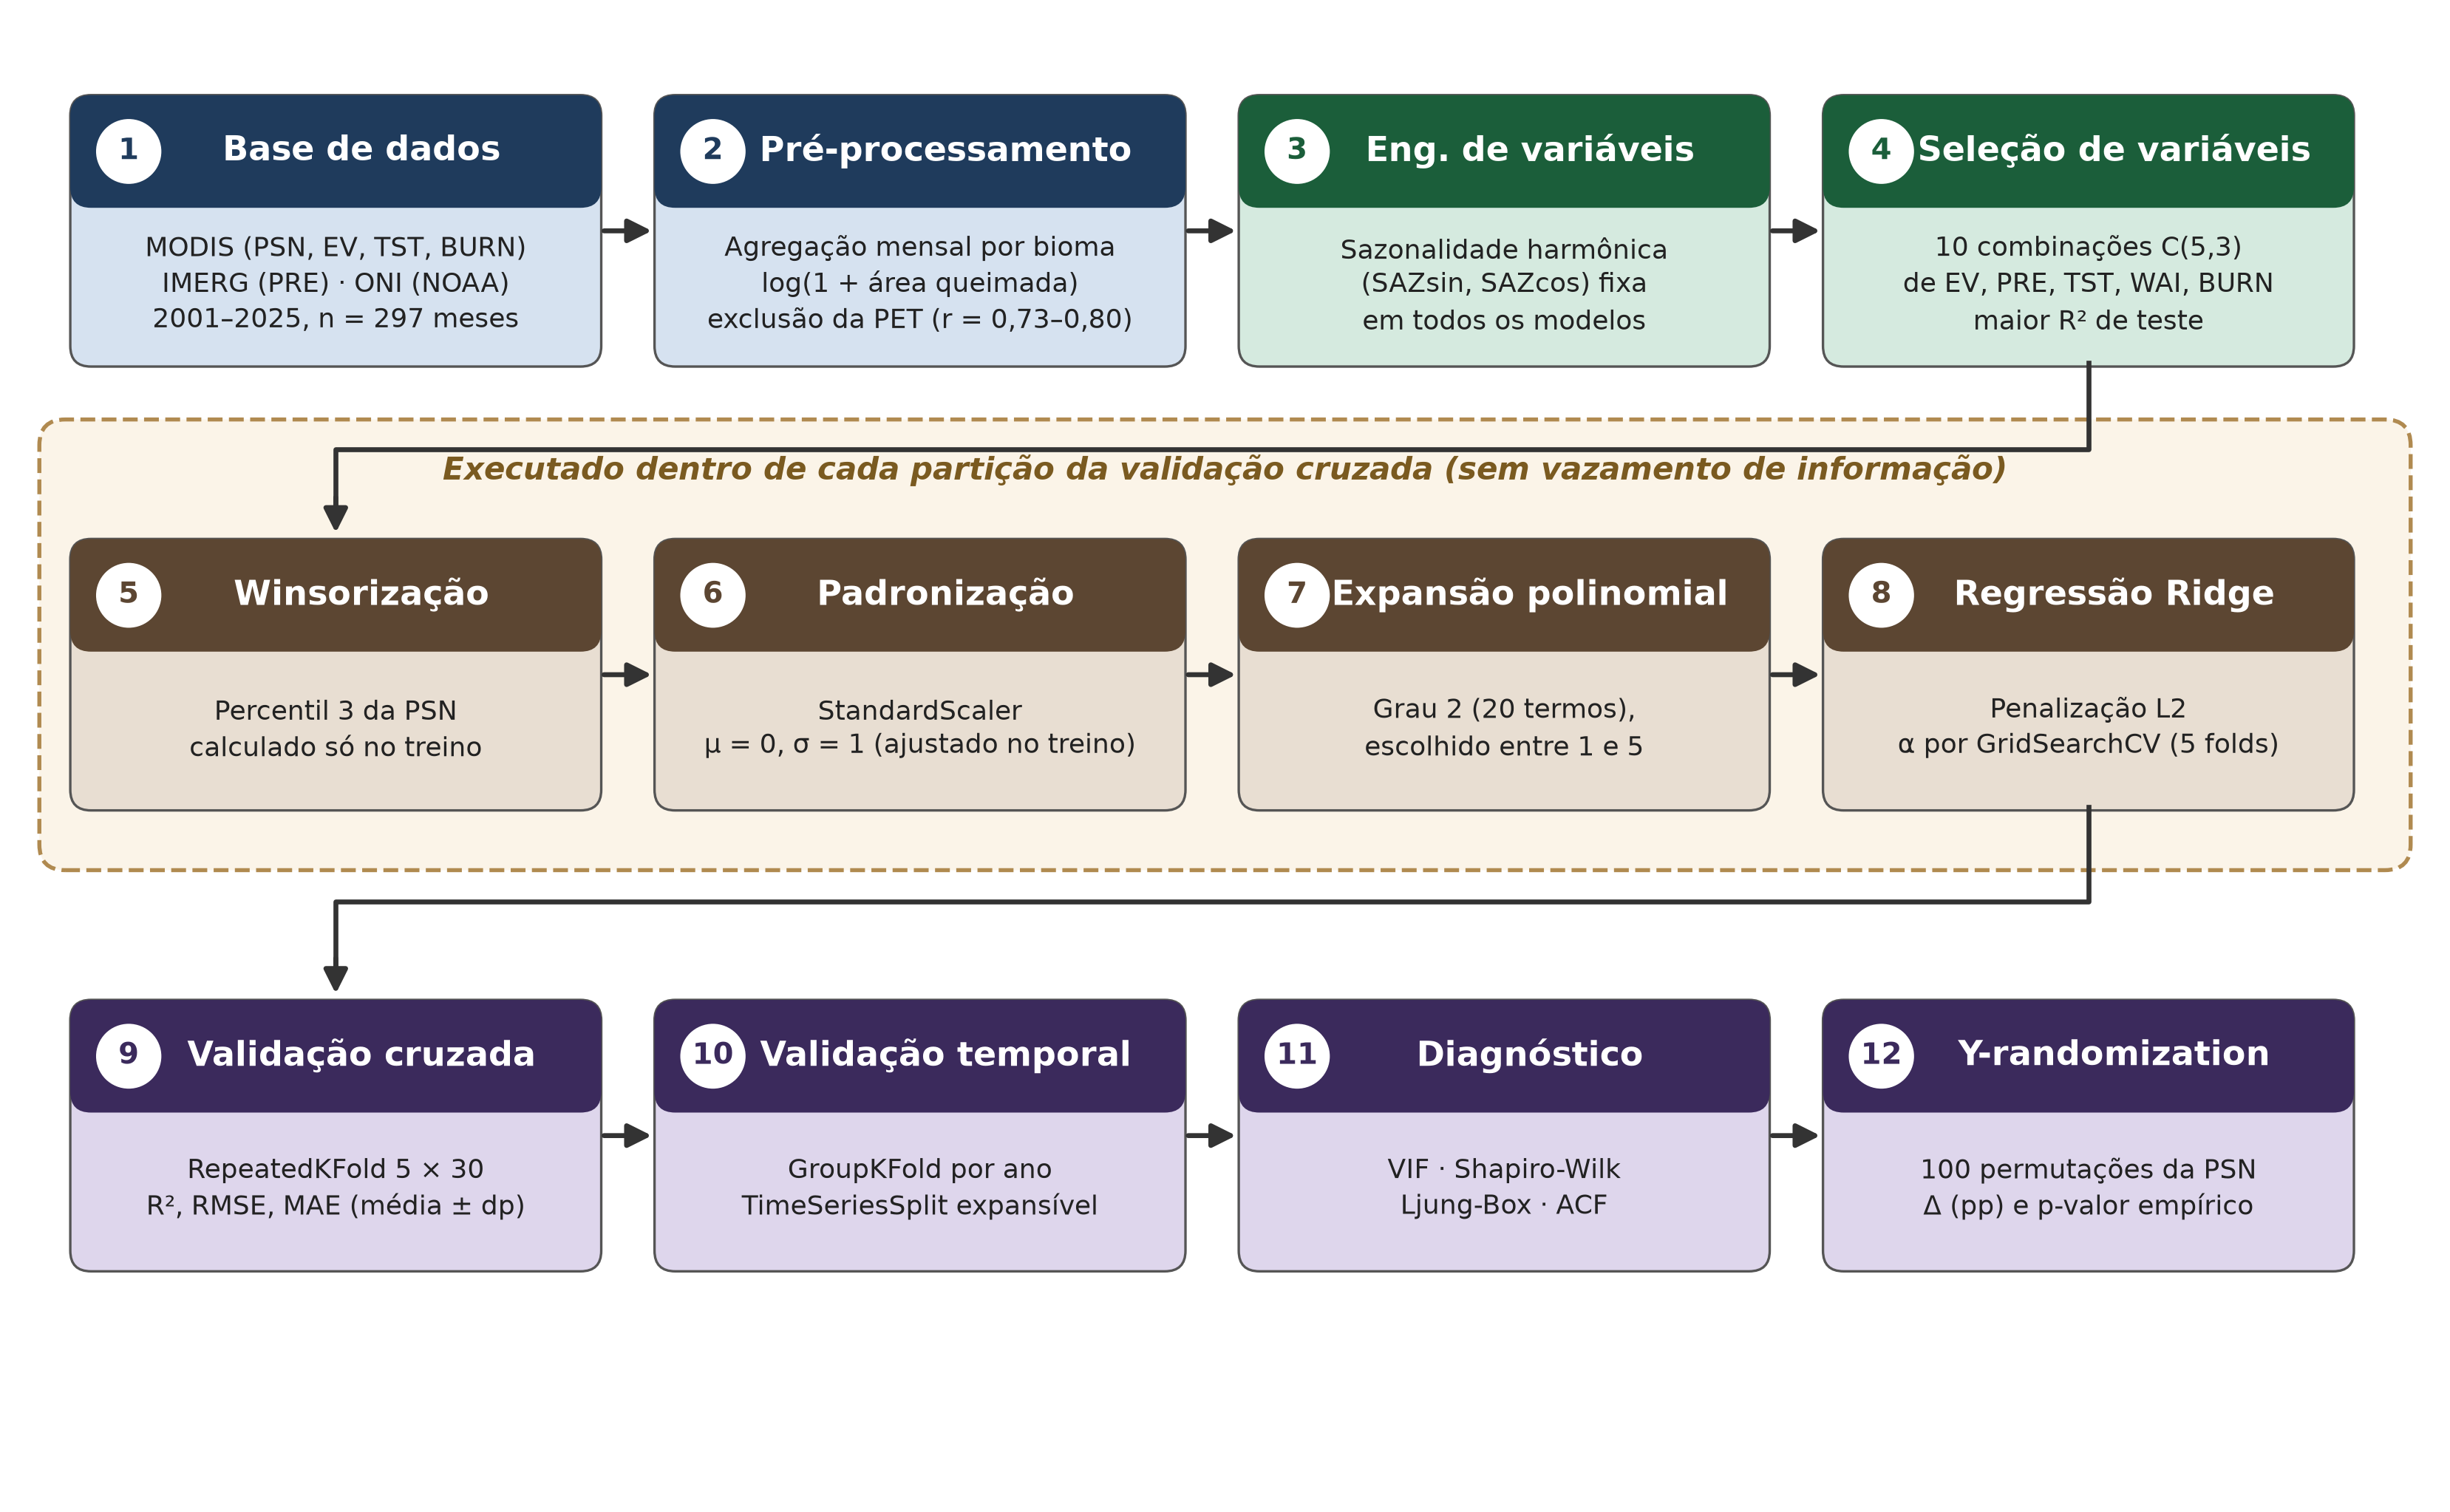
\includegraphics[width=\textwidth]{figs/fig2_workflow.png}
  \caption{Methodological workflow of the MPRM-N. Steps 5 to 8 are executed within each cross-validation partition, without information leakage between training and test sets.}\label{fig:flow}
\end{figure}

\subsection{Model selection, validation and statistical analysis}

Polynomial degree and predictor set were treated as hyperparameters. Degrees 1 to 5 and the $\binom{5}{3} = 10$ combinations of three environmental variables were compared, per biome, by the composite criterion of highest mean test $R^2$ and smallest train--test gap, with 10 percentage points adopted as a guiding reference for overfitting. The main performance estimate came from RepeatedKFold cross-validation with five folds and thirty repetitions (150 partitions), reporting the mean and standard deviation of test $R^2$, RMSE and MAE and the empirical 95\% interval of $R^2$, defined by the 2.5th and 97.5th percentiles across partitions. Because neighbouring months share seasonal structure, performance was additionally verified by two schemes: year-grouped GroupKFold, which keeps entire years out of training in five blocks of five years, and TimeSeriesSplit with an expanding window, which fits the model on the past and evaluates it on the following 49 months in five successive blocks. Only the latter strictly preserves chronological order; the former evaluates generalization to unseen years and prevents consecutive, autocorrelated months of the same year from being split between training and test.

The relative contribution index of each variable was computed as the sum of the absolute values of the standardized coefficients of all terms involving that variable, normalized to 100\% per biome; it is a descriptive index of the fitted model, not a causal measure. To assess the role of the harmonic components, the final model of each biome was refitted without them under the same protocol, and the proportion of each predictor's variance explained by the annual cycle was estimated by regression against SAZsin and SAZcos. Multicollinearity was diagnosed by the Variance Inflation Factor (VIF) on the original predictors, with the usual thresholds of 5 and 10 taken as rules of thumb rather than absolute criteria \citep{obrien2007}. Normality of residuals from a fit to the full series was assessed by the Shapiro--Wilk test and autocorrelation by the Ljung--Box test with 12 lags. The Y-randomization test, adapted from \citet{guimaraes2024}, refitted the model 100 times with permuted PSN and compared the original cross-validated $R^2$ with that of the permuted models through two indicators: the distance between the original $R^2$ and the mean of the permuted models, reported descriptively, and a one-sided empirical p-value, defined as the proportion of permutations with $R^2$ equal to or higher than the original, with significance at $p < 0.05$. Because degree and predictor set were chosen on the basis of RepeatedKFold, we checked whether the same choices would be made when the selection itself uses the temporal schemes: degrees 1 to 5 and the 10 combinations were re-evaluated, with the same pipeline, under year-grouped GroupKFold and under TimeSeriesSplit, recording the degree with the highest test $R^2$ and the rank of the selected combination in each scheme. Selection stability was further measured partition by partition in RepeatedKFold: the frequency with which each combination was the best among the 150 partitions and the paired difference in test $R^2$ between the first and second combinations of each biome, with a 95\% confidence interval from a bootstrap of the partitions (5,000 resamples) and a paired Wilcoxon test.

As a complement to the coefficient-based index, whose comparability across terms of different order is limited, permutation importance \citep{breiman2001} was computed in a manner compatible with temporal dependence: in each test block of year-grouped GroupKFold and TimeSeriesSplit, the model fitted on the training block was evaluated on the test block with each original predictor shuffled 20 times, before the polynomial expansion, so that all terms derived from the variable are affected together. The mean drop in test $R^2$ and the ratio between RMSE with and without shuffling measure how much out-of-sample performance depends on each variable; the mean and standard deviation across blocks and the share of each variable in the total drop are reported. Because shuffling a predictor also breaks its correlations with the others, collinear variables share importance, and the measure should be read as predictive, not causal.

Full permutation of PSN in Y-randomization destroys all temporal dependence of the response, which makes the test undemanding for autocorrelated series. The same procedure (cross-validated RepeatedKFold $R^2$ with fixed $\alpha$) was therefore repeated under two null models that keep the autocorrelation and the seasonal cycle of PSN: circular shifting of the PSN series relative to the predictors, for all 296 possible shifts, among which the 24 multiples of 12 months fully preserve the calendar; and permutation of whole years (100 permutations of the 24 complete years, with the nine months of 2025 kept in place). Under these nulls the model still has access to the seasonality and temporal memory of the series; what is lost is the alignment between PSN and the climatic conditions of the same period. The empirical p-value was defined as (number of nulls with $R^2$ equal to or higher than the original + 1)/($n$ + 1). Analyses were performed in Python 3.11 with scikit-learn, statsmodels and scipy, with a fixed random seed; a single run of the model script reproduces the fit and all validations.

\section{Results}\label{sec:results}

\subsection{Predictive performance and polynomial degree}

Univariate relationships between PSN and the predictors differed among biomes. In the Cerrado and Caatinga, evapotranspiration (74.8\% and 76.2\% of PSN variance) and WAI (74.1\% and 81.5\%) were the strongest single predictors, followed by temperature, with a negative relationship (59.2\% and 54.2\%); same-month precipitation explained less than 10\%. In the Atlantic Forest, no single variable explained more than 12.5\% of PSN variance.

The degree-2 MPRM-N reached a test $R^2$ of 96.7\% in the Cerrado, 94.2\% in the Caatinga and 73.7\% in the Atlantic Forest, with RMSE between 6.69 and 7.97~gC\,m$^{-2}$\,month$^{-1}$ and train--test gaps of 0.59, 1.03 and 5.19 percentage points (Table~\ref{tbl:perf}). Fig.~\ref{fig:obspred} shows the agreement between observed and out-of-sample predicted PSN. Under year-grouped validation, $R^2$ remained practically equal to that of the main validation in all biomes; under TimeSeriesSplit, it stayed above 91\% in the Cerrado and Caatinga and fell to 66.98\% in the Atlantic Forest, a maximum drop of 6.66 points (Table~\ref{tbl:perf}). Winsorization at 0\%, 1\%, 3\% or 5\% changed test $R^2$ by at most 1.3 points in any biome.

\begin{table}[htbp]
\caption{Predictive performance of the degree-2 MPRM-N by biome: mean test $R^2$ ($\pm$ standard deviation) with empirical 95\% interval, RMSE and MAE (gC\,m$^{-2}$\,month$^{-1}$) and train--test gap under RepeatedKFold $5 \times 30$, and test $R^2$ under the temporal validation schemes. All sets include SAZsin and SAZcos.}\label{tbl:perf}
\footnotesize
\begin{tabular*}{\tblwidth}{@{}LLCCCCCCC@{}}
\toprule
Biome & Selected set & Test $R^2$ (\%) & Emp. 95\% (\%) & RMSE & MAE & Gap (pp) & Year-grouped (\%) & Chronological (\%) \\
\midrule
Atlantic Forest & EV + LST + WAI & 73.7 $\pm$ 5.9 & 60.1--83.4 & 7.97 & 6.29 & 5.19 & 73.73 & 66.98 \\
Cerrado & EV + PRE + WAI & 96.7 $\pm$ 0.6 & 95.4--97.7 & 6.74 & 5.43 & 0.59 & 96.38 & 95.73 \\
Caatinga & EV + PRE + LST & 94.2 $\pm$ 1.5 & 90.8--96.2 & 6.69 & 5.08 & 1.03 & 93.81 & 91.20 \\
\bottomrule
\end{tabular*}
\end{table}

\begin{figure}
  \centering
  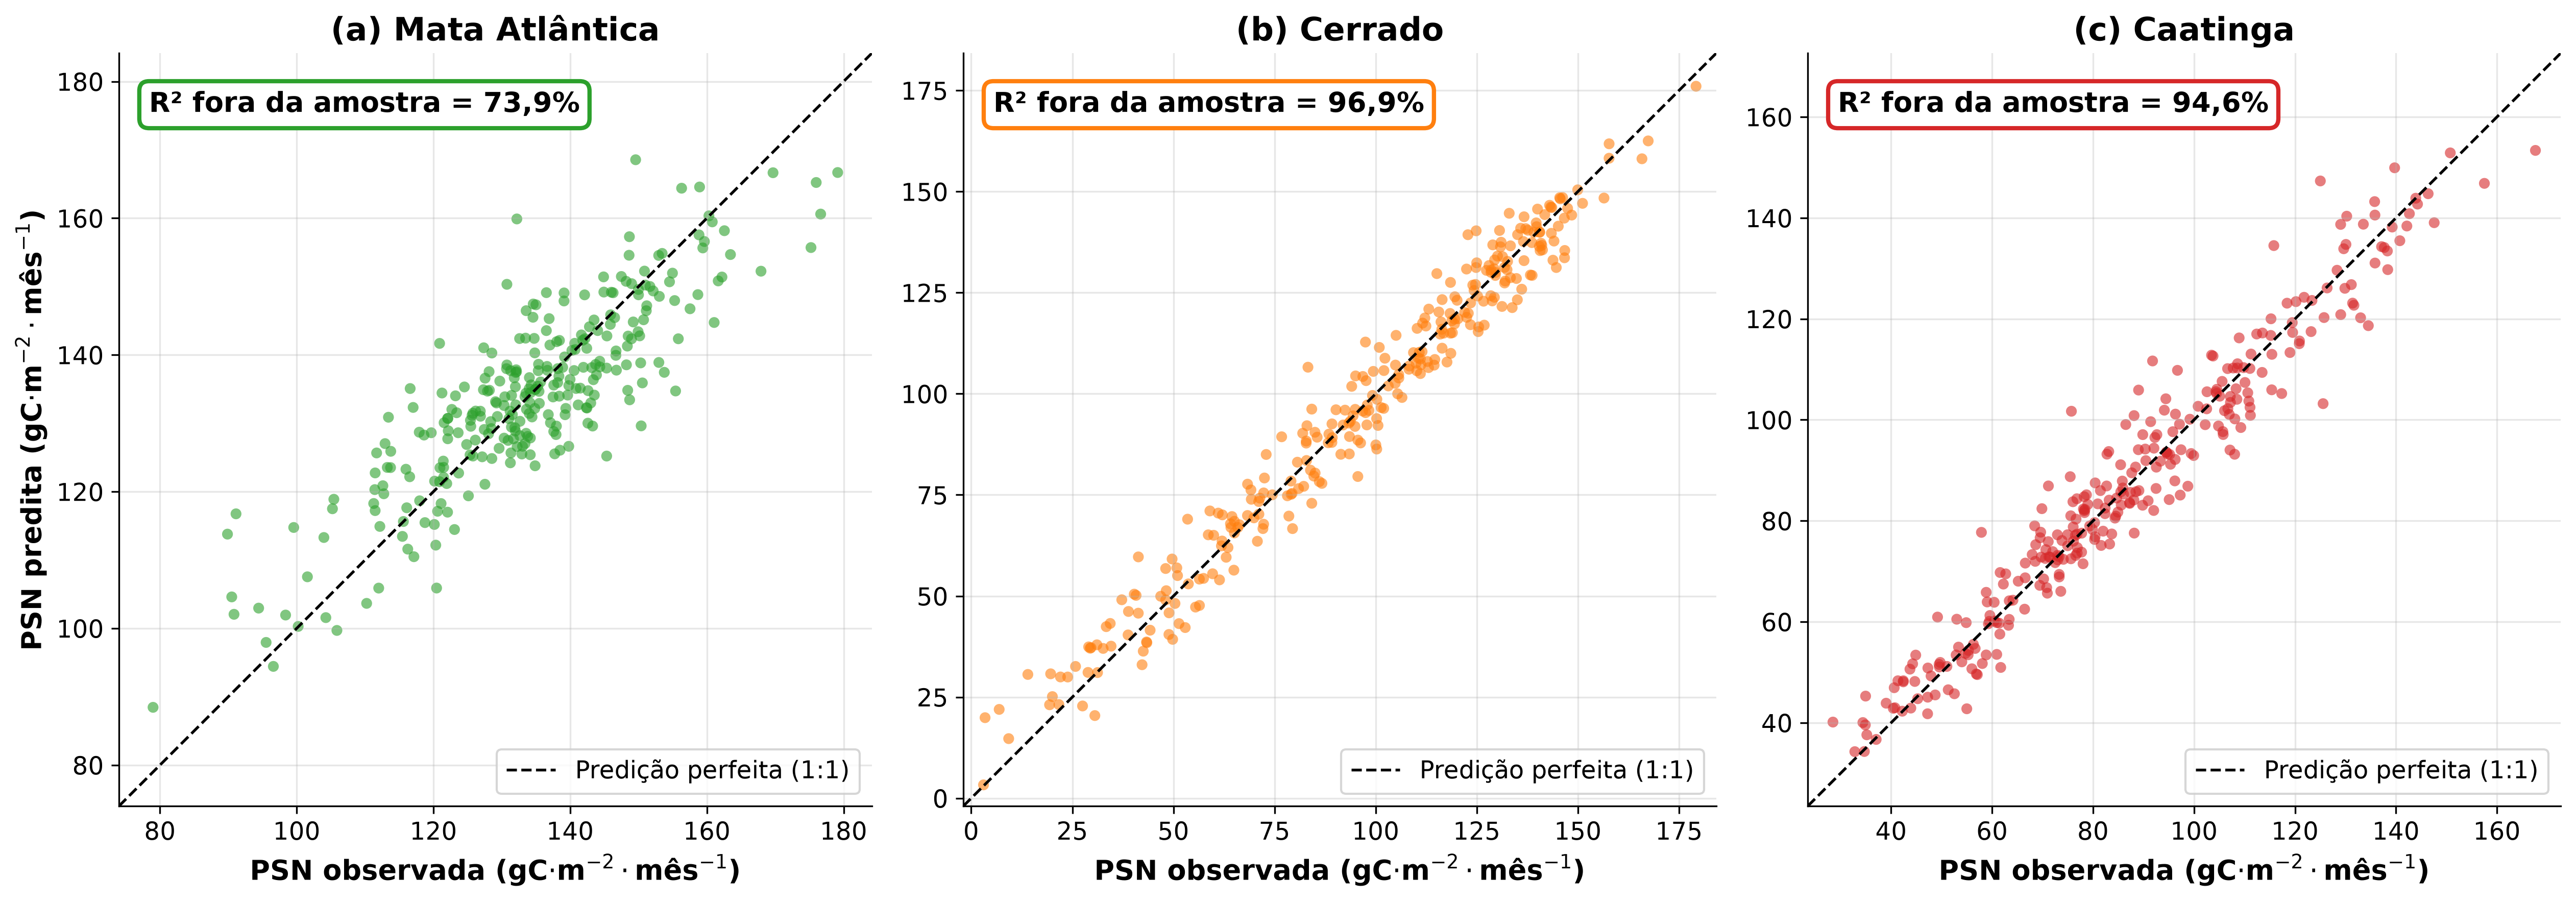
\includegraphics[width=\textwidth]{figs/fig3_obspred.png}
  \caption{Observed (MOD17A2HGF) and MPRM-N predicted PSN in the three biomes, with out-of-sample predictions from five-fold cross-validation.}\label{fig:obspred}
\end{figure}

Degree 2 offered the best compromise between test performance, stability and parsimony in all three biomes (Fig.~\ref{fig:degree}). The gain over the linear model was 8.4 points of test $R^2$ in the Atlantic Forest (65.2\% to 73.6\%), 6.6 points in the Cerrado (90.1\% to 96.7\%) and 1.3 points in the Caatinga (92.9\% to 94.2\%). In the Atlantic Forest, degree 3 reached an $R^2$ 0.8 points higher than degree 2, with a train--test gap 1.7 points larger and 55 terms instead of 20, and was set aside by the composite criterion. At degrees 4 and 5, test $R^2$ decreased and the train--test gap reached tens to hundreds of points. Degree selection did not depend on the validation scheme (Table~\ref{tbl:degtemp}). Repeated under year-grouped GroupKFold and TimeSeriesSplit, the comparison identified degree 2 as the highest test $R^2$ in the Cerrado under both schemes, and in the remaining cases the advantage of another degree did not exceed 0.8 points: degree 3 in the Atlantic Forest under GroupKFold (74.5\% against 73.7\%) and degree 1 in the Caatinga under TimeSeriesSplit (91.5\% against 91.2\%), both within the variation across partitions. Degrees 4 and 5 degraded performance under all schemes.

\begin{table}[htbp]
\caption{Test $R^2$ (\%) of the MPRM-N by polynomial degree under the three validation schemes, with the selected predictor set of each biome.}\label{tbl:degtemp}
\footnotesize
\begin{tabular*}{\tblwidth}{@{}LCCCCC@{}}
\toprule
Biome / scheme & Degree 1 & Degree 2 & Degree 3 & Degree 4 & Degree 5 \\
\midrule
Atlantic Forest, RepeatedKFold & 65.2 & 73.6 & 74.4 & 68.4 & 65.1 \\
Atlantic Forest, year-grouped GroupKFold & 65.5 & 73.7 & 74.5 & 67.4 & 67.2 \\
Atlantic Forest, TimeSeriesSplit & 58.7 & 67.0 & 61.0 & 56.3 & 53.9 \\
Cerrado, RepeatedKFold & 90.1 & 96.7 & 96.4 & 96.1 & 93.7 \\
Cerrado, year-grouped GroupKFold & 90.0 & 96.4 & 96.2 & 96.1 & 95.8 \\
Cerrado, TimeSeriesSplit & 88.5 & 95.7 & 93.7 & 93.4 & 92.2 \\
Caatinga, RepeatedKFold & 92.9 & 94.2 & 93.4 & 63.8 & 52.3 \\
Caatinga, year-grouped GroupKFold & 92.8 & 93.8 & 92.8 & 91.3 & 85.2 \\
Caatinga, TimeSeriesSplit & 91.5 & 91.2 & 90.4 & 87.0 & 86.7 \\
\bottomrule
\end{tabular*}
\end{table}

\begin{figure}
  \centering
  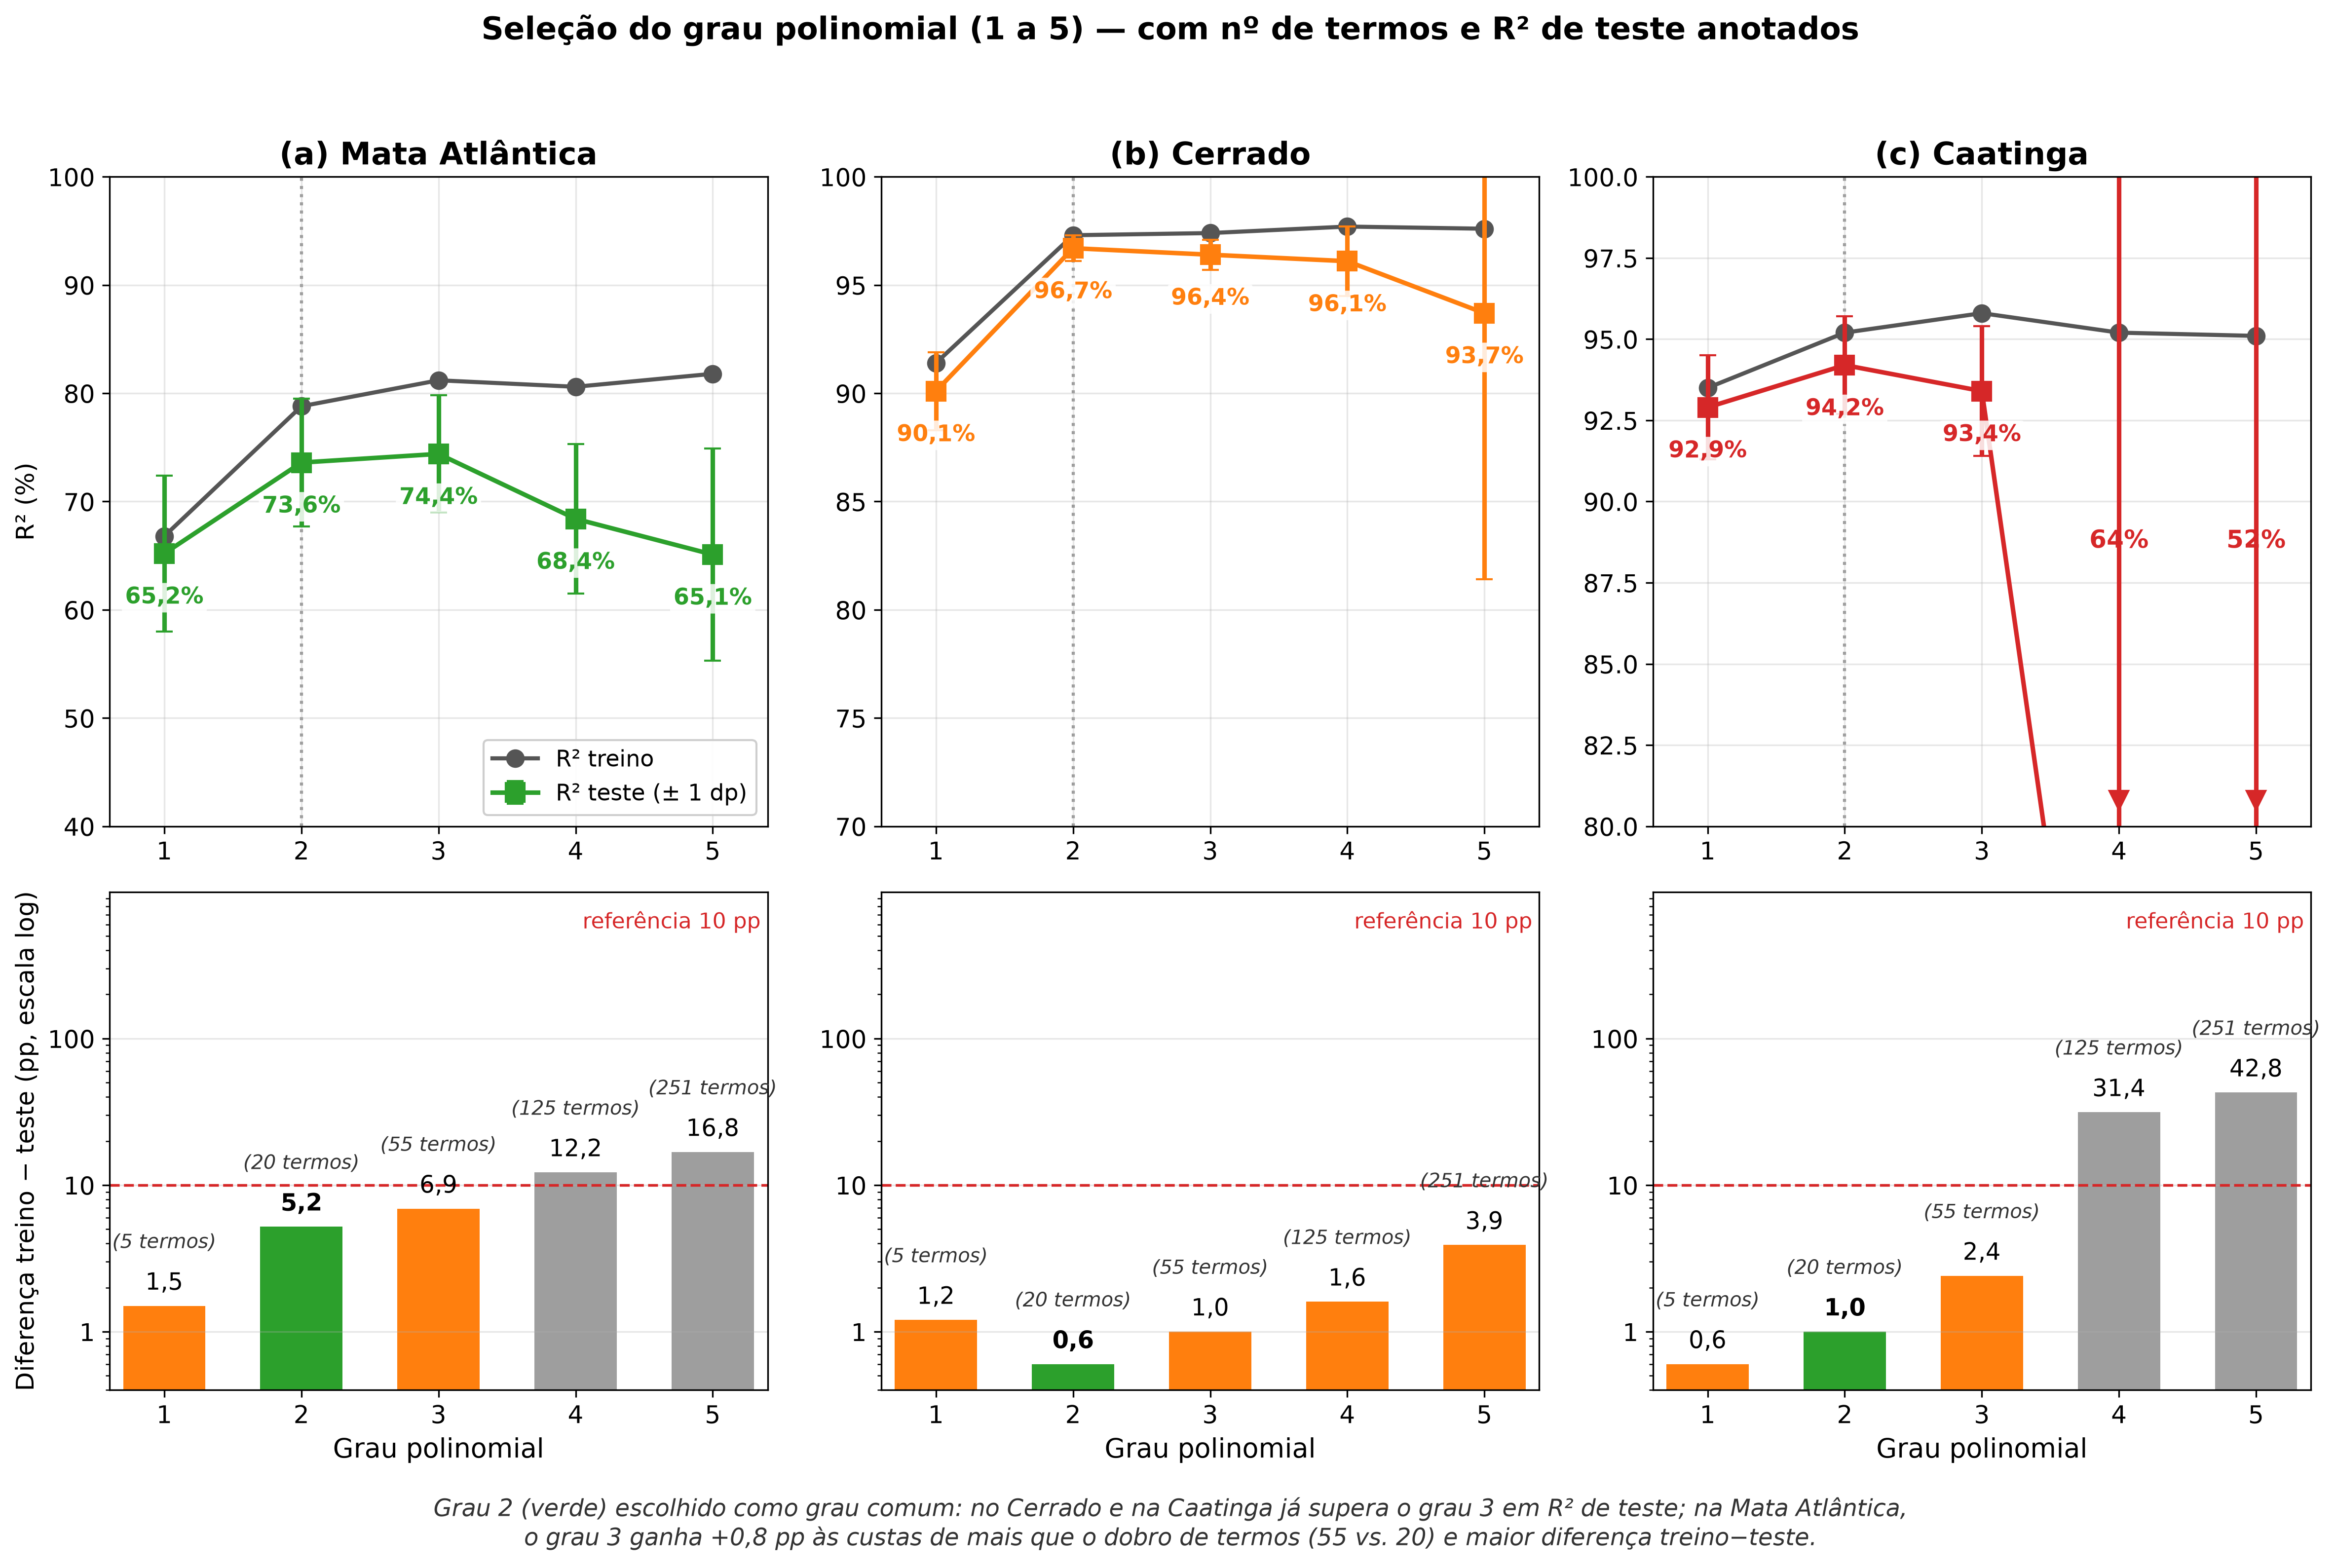
\includegraphics[width=\textwidth]{figs/fig4_degree.png}
  \caption{Selection of the polynomial degree of the MPRM-N in the three biomes: training and test $R^2$ and train--test gap by degree (RepeatedKFold $5 \times 30$).}\label{fig:degree}
\end{figure}

\subsection{Predictor sets and relative contribution}

The selected predictor sets differed among biomes (Table~\ref{tbl:sets}). In the Cerrado, the set EV + PRE + WAI had the smallest train--test gap of all combinations and was the best in 83\% of the 150 partitions; its paired difference in test $R^2$ relative to EV + PRE + LST was 0.39 points (bootstrap 95\% CI: 0.33 to 0.45; Wilcoxon, $p < 0.001$), positive in 86\% of the partitions, and the set also ranked first under year-grouped GroupKFold and TimeSeriesSplit. In the Atlantic Forest, EV + LST + WAI was the best in 66\% of the partitions and ranked first under both temporal schemes. In the Caatinga, the three best combinations were separated by less than 0.3 points: EV + PRE + LST was the best in 36\% of the partitions and ranked first under GroupKFold and second under TimeSeriesSplit, behind EV + PRE + WAI (91.9\% against 91.2\%), making it the least stable choice of the three biomes. In the Atlantic Forest, the set EV + LST + WAI exceeded the combination EV + PRE + LST by 2.7 points, although WAI alone explains less than 2\% of PSN variance in that biome. Burned area was not part of the selected set in any biome. Evapotranspiration had the highest relative contribution index in all biomes (26.9\% in the Atlantic Forest, 37.4\% in the Cerrado and 42.8\% in the Caatinga), and the harmonic components together accounted for 32\% to 40\% of the index in each biome (Fig.~\ref{fig:contrib}).

\begin{table}[htbp]
\caption{Three best combinations of environmental variables per biome (plus SAZsin and SAZcos), degree 2: training and test $R^2$ and train--test gap under RepeatedKFold $5 \times 30$, frequency with which the combination was the best among the 150 partitions, and rank under year-grouped GroupKFold and TimeSeriesSplit.}\label{tbl:sets}
\footnotesize
\begin{tabular*}{\tblwidth}{@{}LLCCCCCC@{}}
\toprule
Biome & Variables & Training $R^2$ (\%) & Test $R^2$ (\%) & Gap (pp) & Best in (\%) & Year-grouped rank & Chronological rank \\
\midrule
Atlantic Forest & EV + LST + WAI & 78.8 & 73.6 & 5.2 & 66.0 & 1st & 1st \\
 & EV + PRE + LST & 76.1 & 71.0 & 5.1 & 19.3 & 2nd & 2nd \\
 & EV + PRE + WAI & 74.4 & 69.0 & 5.4 & 12.0 & 3rd & 3rd \\
Cerrado & EV + PRE + WAI & 97.3 & 96.7 & 0.6 & 82.7 & 1st & 1st \\
 & EV + PRE + LST & 97.0 & 96.3 & 0.7 & 14.0 & 2nd & 2nd \\
 & EV + PRE + BURN & 96.9 & 95.8 & 1.2 & 2.7 & 3rd & 3rd \\
Caatinga & EV + PRE + LST & 95.2 & 94.2 & 1.0 & 36.0 & 1st & 2nd \\
 & EV + PRE + WAI & 95.1 & 94.0 & 1.1 & 22.0 & 2nd & 1st \\
 & PRE + LST + WAI & 95.0 & 93.9 & 1.1 & 28.7 & 4th & 5th \\
\bottomrule
\end{tabular*}
\end{table}

\begin{figure}
  \centering
  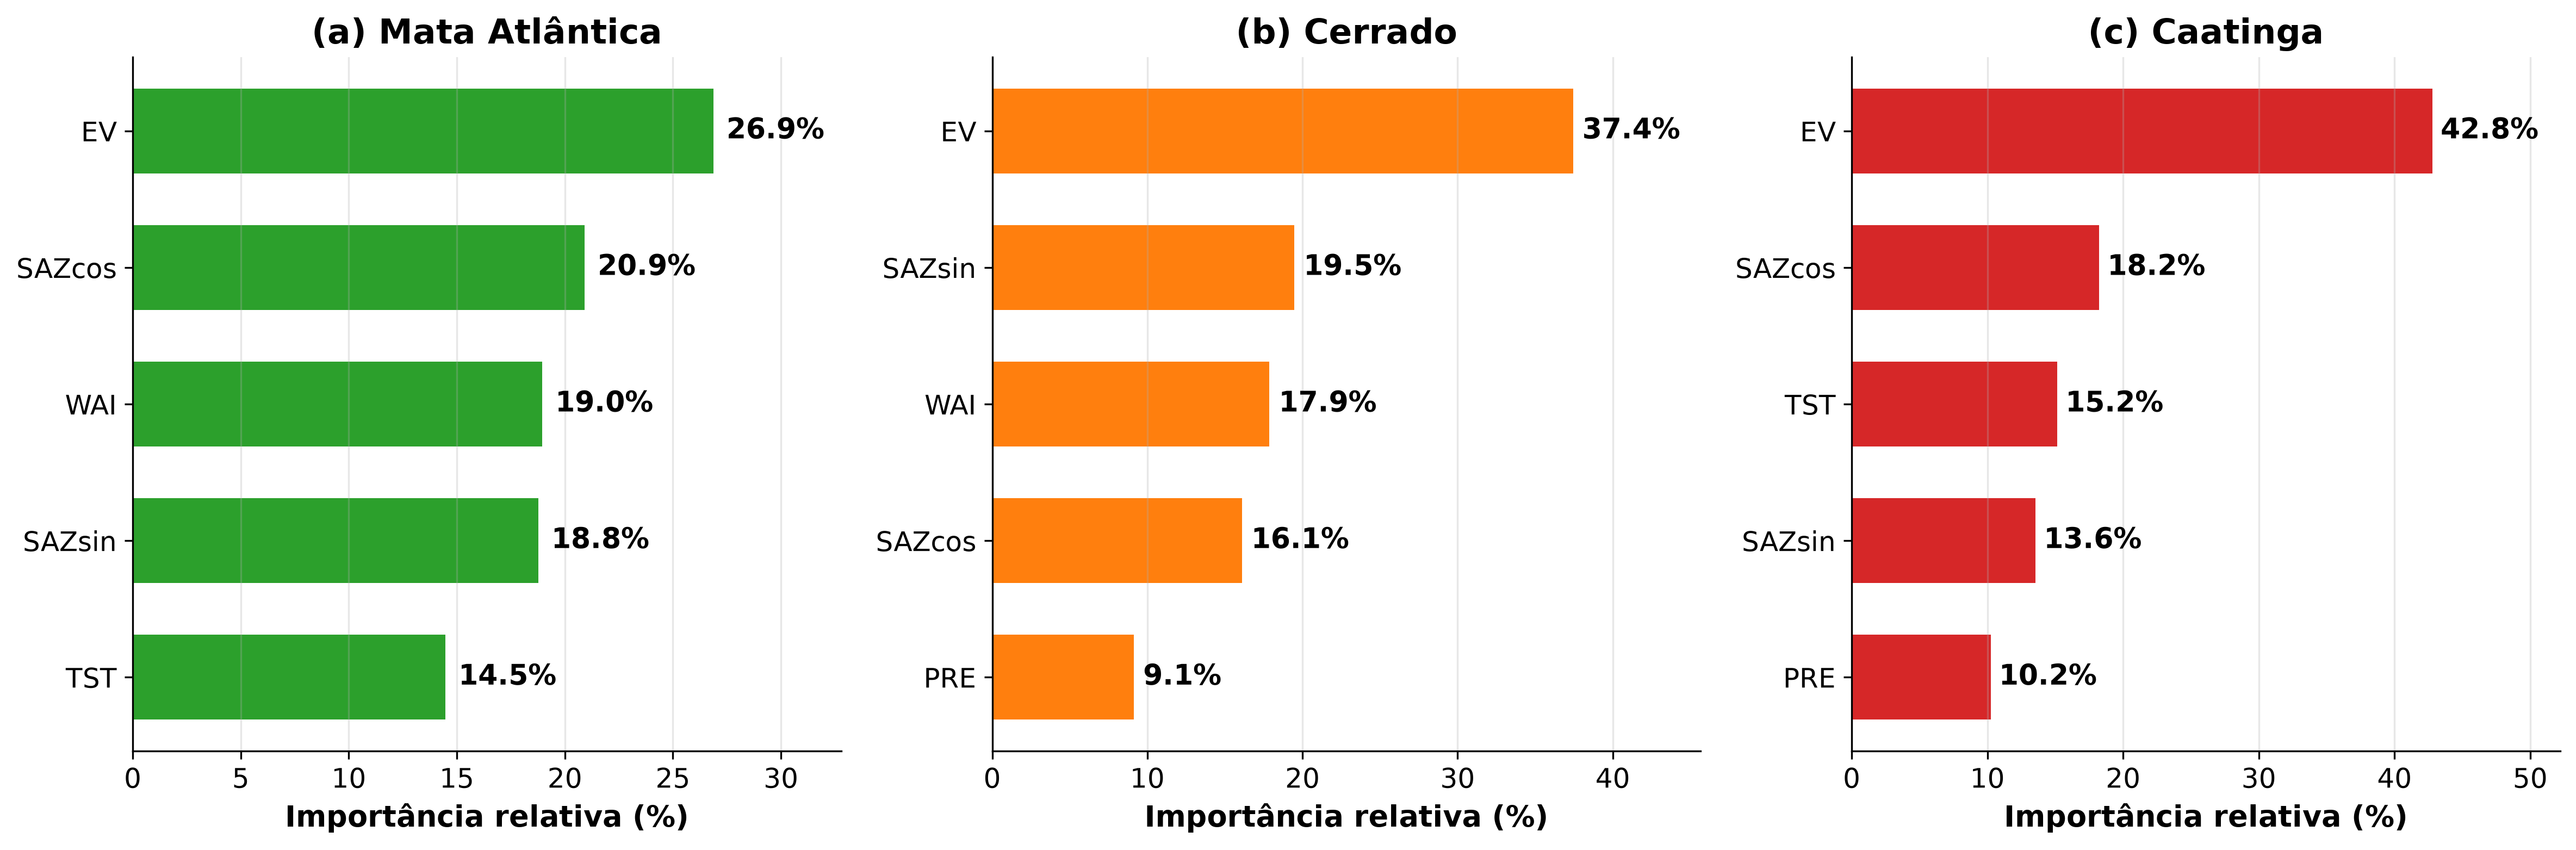
\includegraphics[width=\textwidth]{figs/fig5_contribution.png}
  \caption{Relative contribution index of the predictor variables in the degree-2 MPRM-N in the three biomes.}\label{fig:contrib}
\end{figure}

Out-of-sample permutation importance (Table~\ref{tbl:perm}) agreed with the coefficient index on the dominant predictor, evapotranspiration, but assigned it a much larger share: 42\% of the total drop in $R^2$ in the Atlantic Forest, 85\% in the Cerrado and 80\% in the Caatinga under year-grouped GroupKFold, with similar shares under TimeSeriesSplit. The two measures diverged for the secondary variables: in the Cerrado, WAI received 3\% of the total drop under permutation, against 18\% in the coefficient index, because much of its information is shared with EV. The absolute drops are large because shuffling a central predictor drives the quadratic and interaction terms to extrapolate.

\begin{table}[htbp]
\caption{Out-of-sample permutation importance: share of each variable in the total drop of test $R^2$ (\%, mean $\pm$ standard deviation across the five blocks, 20 shuffles per block) and ratio between RMSE with and without shuffling, under year-grouped GroupKFold and TimeSeriesSplit.}\label{tbl:perm}
\footnotesize
\begin{tabular*}{\tblwidth}{@{}LLCCCC@{}}
\toprule
Biome & Variable & Year-grouped share (\%) & Year-grouped RMSE ratio & Chronological share (\%) & Chronological RMSE ratio \\
\midrule
Atlantic Forest & EV & 41.9 $\pm$ 7.7 & 4.16 & 38.2 $\pm$ 6.4 & 3.47 \\
 & WAI & 21.1 $\pm$ 5.0 & 3.01 & 19.9 $\pm$ 5.1 & 2.64 \\
 & SAZcos & 16.6 $\pm$ 2.5 & 2.74 & 16.7 $\pm$ 2.7 & 2.43 \\
 & SAZsin & 11.0 $\pm$ 1.2 & 2.29 & 15.2 $\pm$ 3.8 & 2.34 \\
 & LST & 9.4 $\pm$ 3.8 & 2.10 & 10.0 $\pm$ 4.5 & 1.89 \\
Cerrado & EV & 85.3 $\pm$ 1.4 & 11.25 & 77.7 $\pm$ 15.1 & 10.24 \\
 & SAZcos & 4.4 $\pm$ 0.6 & 2.74 & 6.1 $\pm$ 3.6 & 2.70 \\
 & PRE & 4.1 $\pm$ 0.8 & 2.62 & 3.7 $\pm$ 0.4 & 2.41 \\
 & SAZsin & 3.6 $\pm$ 0.6 & 2.50 & 5.0 $\pm$ 1.9 & 2.59 \\
 & WAI & 2.6 $\pm$ 0.9 & 2.15 & 7.5 $\pm$ 10.2 & 2.46 \\
Caatinga & EV & 80.4 $\pm$ 2.5 & 6.81 & 76.9 $\pm$ 10.0 & 5.13 \\
 & SAZcos & 8.9 $\pm$ 1.5 & 2.48 & 4.7 $\pm$ 2.3 & 1.65 \\
 & SAZsin & 4.6 $\pm$ 1.0 & 1.90 & 3.2 $\pm$ 1.5 & 1.47 \\
 & LST & 3.7 $\pm$ 1.2 & 1.75 & 11.4 $\pm$ 13.4 & 1.82 \\
 & PRE & 2.4 $\pm$ 1.2 & 1.48 & 3.8 $\pm$ 2.3 & 1.42 \\
\bottomrule
\end{tabular*}
\end{table}

\subsection{Role of the harmonic components}

Removing the harmonic components lowered test $R^2$ by 21.8 points in the Atlantic Forest, 3.0 points in the Cerrado and 2.4 points in the Caatinga (Table~\ref{tbl:harm}). In the Cerrado, 70\% to 79\% of the variance of evapotranspiration and WAI was explained by the annual cycle, against about 40\% in the Atlantic Forest. With harmonics present, the contribution of precipitation fell from 29.0\% to 9.1\% in the Cerrado and from 24.1\% to 10.2\% in the Caatinga, and that of temperature fell from 40.3\% to 14.5\% in the Atlantic Forest, whereas the contribution of evapotranspiration was maintained or increased. The correlation between monthly anomalies of evapotranspiration and of PSN ranged from 0.73 to 0.93, while that of precipitation was 0.02 in the Cerrado and 0.16 in the Caatinga.

\begin{table}[htbp]
\caption{Effect of the harmonic components: test $R^2$ of the MPRM-N with and without explicit seasonality, proportion of each predictor's variance explained by the annual cycle, correlation of monthly anomalies with PSN, and relative contribution index without and with harmonics. Harmonics received 32\% to 40\% of the total index in each biome. Anomaly = deviation from the calendar-month mean over the series.}\label{tbl:harm}
\scriptsize
\begin{tabular*}{\tblwidth}{@{}LCLCCCC@{}}
\toprule
Biome & $R^2$ with / without (\%) & Variable & Annual-cycle $R^2$ (\%) & $r$ anomalies & Index without (\%) & Index with (\%) \\
\midrule
Atlantic Forest & 73.7 / 51.9 & EV & 39.8 & 0.73 & 27.0 & 26.9 \\
 & & LST & 64.9 & $-$0.58 & 40.3 & 14.5 \\
 & & WAI & 39.8 & 0.42 & 32.8 & 19.0 \\
Cerrado & 96.7 / 93.7 & EV & 79.1 & 0.90 & 34.7 & 37.4 \\
 & & PRE & 58.9 & 0.02 & 29.0 & 9.1 \\
 & & WAI & 70.2 & 0.76 & 36.2 & 17.9 \\
Caatinga & 94.2 / 91.8 & EV & 63.3 & 0.93 & 49.5 & 42.8 \\
 & & PRE & 31.5 & 0.16 & 24.1 & 10.2 \\
 & & LST & 54.2 & $-$0.77 & 26.4 & 15.2 \\
\bottomrule
\end{tabular*}
\end{table}

\subsection{Diagnostics, Y-randomization and temporal nulls}

VIF was below 5.1 for all predictors in the Atlantic Forest and Caatinga; in the Cerrado, evapotranspiration and WAI had VIF of 36.99 and 31.61. Residuals were normal in the Atlantic Forest (Shapiro--Wilk, $p = 0.630$) and Cerrado ($p = 0.423$) and showed a left-tail deviation in the Caatinga ($p = 0.002$). The Ljung--Box test detected residual autocorrelation in all biomes ($p \le 0.005$), with lag-1 autocorrelation of 0.51 in the Atlantic Forest, 0.20 in the Cerrado and 0.42 in the Caatinga. In the Y-randomization test, models fitted to permuted PSN had mean cross-validated $R^2$ of $-10.6\%$, $-10.9\%$ and $-13.0\%$, against 73.8\%, 96.7\% and 94.2\% for the original models, distances of 84.4, 107.5 and 107.2 points; none of the 100 permutations matched the original model ($p = 0.0099$). Under the nulls that preserve the temporal structure (Table~\ref{tbl:nulls}), the null models reached mean $R^2$ values well above those of free permutation, especially with the permutation of whole years (62.4\% in the Cerrado and 40.2\% in the Caatinga), which keeps the seasonality and memory of the series, but no null reached the original model in any biome (empirical $p$ between 0.003 and 0.040).

\begin{table}[htbp]
\caption{Null models preserving the temporal structure of PSN: cross-validated $R^2$ (RepeatedKFold $5 \times 30$, fixed $\alpha$) of the original model and of the null models obtained by circular shifting of PSN (all 296 shifts and the subset of multiples of 12 months) and by permutation of whole years (100 permutations). Empirical $p$ = (number of nulls with $R^2 \ge$ original + 1)/($n$ + 1).}\label{tbl:nulls}
\footnotesize
\begin{tabular*}{\tblwidth}{@{}LLCCCCC@{}}
\toprule
Biome & Null & $n$ & Original $R^2$ (\%) & Null $R^2$, mean $\pm$ sd (\%) & Null $R^2$, max.\ (\%) & Empirical $p$ \\
\midrule
Atlantic Forest & Circular shift & 296 & 73.8 & $-$3.0 $\pm$ 6.1 & 52.4 & 0.003 \\
 & Shift by multiples of 12 months & 24 & 73.8 & $-$3.2 $\pm$ 5.0 & 7.3 & 0.040 \\
 & Permutation of years & 100 & 73.8 & 4.4 $\pm$ 2.7 & 11.5 & 0.010 \\
Cerrado & Circular shift & 296 & 96.7 & 36.3 $\pm$ 12.9 & 81.8 & 0.003 \\
 & Shift by multiples of 12 months & 24 & 96.7 & 35.5 $\pm$ 11.0 & 58.7 & 0.040 \\
 & Permutation of years & 100 & 96.7 & 62.4 $\pm$ 1.4 & 67.0 & 0.010 \\
Caatinga & Circular shift & 296 & 94.2 & 23.9 $\pm$ 8.9 & 72.5 & 0.003 \\
 & Shift by multiples of 12 months & 24 & 94.2 & 22.5 $\pm$ 7.4 & 36.5 & 0.040 \\
 & Permutation of years & 100 & 94.2 & 40.2 $\pm$ 2.3 & 44.7 & 0.010 \\
\bottomrule
\end{tabular*}
\end{table}

\section{Discussion}\label{sec:discussion}

\subsection{Climatic associations of net photosynthesis in the biomes}

The three biomes form a gradient of climatic predictability of PSN. The high performance in the Cerrado reflects the strong hydrological seasonality of the biome, in which the alternation of dry and wet seasons imposes a regular rhythm on photosynthetic activity; flux-tower studies show that Cerrado primary productivity tracks soil water content and precipitation \citep{arruda2016,biudes2021,vourlitis2022}. In the Caatinga, predictability derives from the resource-pulse regime typical of semi-arid environments, in which vegetation responds almost immediately to rainfall events \citep{schwinning2004,mendes2025,silva2026}, consistent with the marginal gain of degree 2 over the linear model in this biome. The lower performance in the Atlantic Forest reflects the diversity of climate types along the coast \citep{alvares2013} and the structural heterogeneity of the most fragmented biome of the state, where deforestation history, eucalyptus silviculture and edge effects introduce sources of variability that regional climatic predictors cannot capture \citep{lima2020,broggio2024}. \citet{benfica2023} had already observed, in the same series, stronger correlations between PSN and hydrological variables in the Cerrado and Caatinga and weaker seasonal variation in the Atlantic Forest; the present results quantify that difference as a predictability gradient and organize it into three association patterns: seasonal water limitation in the Cerrado, pulsed response to rainfall in the Caatinga and multifactorial response in the Atlantic Forest.

The most relevant outcome of variable selection was the choice of WAI in place of LST in the best-performing combination of the Cerrado. The preference is statistically consistent, with a positive paired difference in 86\% of the partitions and first rank under all three validation schemes, but small in magnitude, 0.4 points of $R^2$; the result therefore indicates redundancy of temperature in the presence of WAI, not its ecological irrelevance. Moreover, because EV and WAI share much of their information in this biome (VIF above 30) and WAI receives only 3\% of the permutation importance, their individual contributions should be read with caution. In the Cerrado, temperature acts primarily through the water balance, raising evaporative demand and reducing soil water availability, a decisive process for the physiology of savanna vegetation \citep{bucci2008,arruda2016}. WAI, defined as the ratio of actual to potential evapotranspiration, expresses the degree to which atmospheric water demand is met by the water available in the system and integrates, in a single variable, the combined effects of temperature and precipitation. The literature on tropical savannas points to seasonal water limitation, rather than thermal limitation, as the main control of productivity \citep{vourlitis2022}. Under projections of intensified droughts and higher evaporative demand for central Brazil \citep{ipcc2022}, and given that productivity responds non-linearly to water availability \citep{mwangi2025}, WAI constitutes a quantitative indicator of climatic vulnerability of the Bahian Cerrado that can be used to monitor productivity trends.

A caveat about data provenance applies to the association between PSN and evapotranspiration. PSN (MOD17A2HGF) and EV (MOD16A2GF) are estimated by algorithms of the same family that share inputs: both use the fraction of absorbed photosynthetically active radiation and the leaf area index from MOD15A2H, the land-cover classification from MCD12Q1 and the same GMAO/MERRA-2 reanalysis meteorology \citep{running2004,running2021gpp,running2021et}. Part of the strong association between EV and PSN observed in the three biomes may therefore reflect algorithmic dependence between the products rather than only the ecophysiological coupling between transpiration and carbon assimilation through the stomata \citep{lawson2019}. This dependence does not invalidate the use of the model for its intended purpose, which is to represent and predict MOD17 PSN from variables available at the same scale; the association of PSN with precipitation (IMERG) and land surface temperature (MOD11A2), products independent of MOD17, points in the same direction, as does the variation of the univariate association from 12.5\% in the Atlantic Forest to 76\% in the Caatinga, which would not occur if the shared algorithm were the dominant factor. It does, however, call for caution in interpreting the magnitude of the EV contribution as autonomous ecological evidence. Validation of the relationships with independent data, such as the eddy-covariance flux measurements available for the Caatinga \citep{mendes2020,mendes2025} and the Cerrado \citep{vourlitis2022}, is indicated as a future step.

In the Atlantic Forest, WAI entered the selected set and received 19\% of the contribution index despite explaining less than 2\% of PSN on its own. This contribution arises exclusively through interactions with evapotranspiration and temperature: in a humid biome not limited by water under average conditions, water availability matters only when combined with specific thermal or evaporative-demand conditions. An additive model would not capture this effect, which explains why degree 2 gained most over the linear model precisely in this biome. The absence of burned area from the selected set of any biome indicates that, at the monthly and biome scale adopted, this variable did not add sufficient predictive power relative to the other predictors. This does not imply absence of an ecological effect of fire, documented in Bahia by \citet{benfica2022,benfica2023} and in tropical savannas by \citet{navarro2025}, and may reflect the spatial heterogeneity of burning within each biome, lagged productivity responses and information shared with the hydrological predictors.

\subsection{Explicit seasonality, regularization and validation}

The analysis with and without harmonic components offers a contribution that goes beyond the case studied. In monthly productivity series, much of the variance is deterministic: photoperiod, radiation and leaf phenology impose an annual cycle that any seasonal climatic variable partly reproduces \citep{wu2016,alberton2019}. When the cycle is not represented explicitly, precipitation and temperature receive credit for the calendar and their contribution is overestimated. When the harmonics absorb the cycle, each predictor is evaluated by the information it adds beyond the typical year, that is, by the anomalies. The results show that same-month rainfall is a noisy and lagged input, with nearly zero correlation with the PSN anomaly in the Cerrado, whereas evapotranspiration measures the water actually used by vegetation and closely tracks the productivity anomaly, because transpiration and carbon assimilation occur through the same stomata \citep{lawson2019}. The sharp loss of performance when seasonality is removed in the Atlantic Forest suggests that PSN in this biome responds to a component of the annual cycle, possibly photoperiod or leaf phenology \citep{borchert2001,wu2016}, not fully represented by the measured climatic variables. Studies of variable contribution in monthly productivity series should therefore include explicit seasonality terms.

The choice of degree 2 in all biomes should be read narrowly: within the variable set and degree range evaluated, quadratic and pairwise interaction terms were sufficient to obtain the best compromise between test performance and model complexity, and higher degrees added no predictive structure that compensated for the increase in terms and overfitting. Regularization was decisive: in the Cerrado, VIF of 37 and 32 for evapotranspiration and WAI would make ordinary least squares estimation unstable, whereas the L2 penalty kept the model stable under all validation schemes. Agreement between repeated cross-validation and the chronological schemes indicates that performance does not derive from neighbouring months falling simultaneously in training and test sets, and the persistence of degree 2 and of the selected sets when the selection itself is performed under the temporal schemes removes the objection that the hyperparameter choice would depend on shuffling the months. The contrast between the coefficient index and permutation importance reinforces the reading of the former as a description of the fitted model structure rather than a measure of importance in the strict sense: the index splits weight among correlated terms, whereas permutation assigns to each variable only the information it carries beyond the others. The nulls that preserve the temporal structure show that seasonality and memory of the series explain, by themselves, a substantial share of $R^2$ in the seasonal biomes, but the difference between the original model and these nulls quantifies the gain that arises from the alignment between PSN and the climatic conditions of the same period, larger in the seasonal biomes and smaller in the Atlantic Forest. The residual autocorrelation detected in all biomes indicates unmodelled temporal memory, such as water stored in the soil \citep{oliveira2005}, and did not prevent predictive capacity from remaining high under chronological validation; the incorporation of lagged predictors or autoregressive terms is the natural extension of the model. Other limitations should be acknowledged: the modelling did not incorporate structural landscape variables, potentially relevant to the residual variability of the Atlantic Forest; the monthly scale limits the representation of short extreme events; the approach is correlational and does not support causal inference; and the model estimates PSN of a month from the variables of the same month, so it does not produce autonomous forecasts. Predictor-set selection was performed on the same partitions used to report performance, not in a fully nested scheme, which may introduce some selection optimism, attenuated by the year-grouped and chronological validations. Three data-provenance limitations should also be stated: PSN and EV come from MODIS algorithms that share inputs; land surface temperature was not filtered by the QC\_Day quality band, and the sensitivity of the series to this filter was not evaluated; and the periods referred to here as monthly are fixed 32-day windows assigned to a reference calendar month. Comparison with generalized additive models and random forests under the same protocol would situate the cost, if any, of the interpretability that the polynomial structure offers.

\section{Conclusions}\label{sec:conclusions}

The degree-2 multiple polynomial regression model, estimated by Ridge regression, explained 96.7\%, 94.2\% and 73.7\% of the monthly variance of PSN in the Cerrado, Caatinga and Atlantic Forest of Bahia between 2001 and 2025, with stable performance under repeated cross-validation, chronological validation and Y-randomization. The selection of degree and predictor sets held when repeated under year-grouped and chronological validation, and performance exceeded null models that preserve the seasonality and autocorrelation of the series. The selected predictor sets differed among biomes: the water availability index was selected in place of temperature in the Cerrado, where it integrates thermal and hydrological information, and contributed through interactions in the Atlantic Forest. Explicit representation of the annual cycle proved essential in the humid biome and changed the interpretation of predictor contribution, which then reflects anomalies rather than the calendar. The three biomes exhibit distinct patterns of association between climate and productivity, which reinforces the need for biome-specific monitoring strategies: in water-limited biomes, a small set of remote-sensing variables is sufficient to track PSN, whereas in the Atlantic Forest the incorporation of structural landscape variables is recommended in future studies. Regularized polynomial regression with empirical selection of degree and variables and temporal validation is a reproducible and interpretable alternative for representing non-linear environmental relationships with satellite data, applicable to other regions with similar environmental gradients.

\section*{Data availability}
The monthly database (297 months per biome, 2001--2025) is provided as supplementary material (CSV file). The Python code and extraction scripts are available in a public repository [insert repository DOI].

\section*{Declaration of competing interest}
The authors declare that they have no known competing financial interests or personal relationships that could have appeared to influence the work reported in this paper.

\section*{Acknowledgements}
This study was financed in part by the Coordenação de Aperfeiçoamento de Pessoal de Nível Superior -- Brasil (CAPES) -- Finance Code 001, through a master's scholarship granted to the first author. The authors thank the Graduate Program in Environmental Sciences and Technologies (UFSB/IFBA). The first author thanks Prof. Dr. Fabrício Berton Zanchi for his supervision and Prof. Dr. Nayanne Silva Benfica for her co-supervision.

\printcredits

\bibliographystyle{cas-model2-names}
\bibliography{refs}

\end{document}
